\chapter{Motivation}
\label{ch:motivation}

Choosing a suitable topic for a Master's Thesis is not a readily decided matter. On one hand a student desires to show some insight into contemporary and maybe even complex problems, but on the other hand the task has to be achievable within a certain timeframe. The project should be theoretical enough to be of interest even for professors while at the same time (at least in Software Development) be practical enough to remaining motivating to the student. In the case of this Thesis I tried to combine scientific and engineering aspects into a project which could be expanded in future endeavors while keeping it sufficiently self contained to represent a work of its own.


\section{Scientific motivation}
\label{sect:scientific_motivation}

Having been a member of the HCI-KDD.org group for over 2 years now, I have developed a genuine interested in graph theory, machine learning, HCI as well as their applications in modern information systems - not least in the context of biomedical applications. Although finalizing my Master's study at a relatively advanced age, I am still open to pursuing a PhD in those areas. Therefore, it seemed logical to tackle some problems related to those fields; however significant progress in such matters are not easily achieved even by professional scientists, leave alone a single MSc student on a deadline...

For this reason I intended to contribute to the future work of Professor Holzingers Team by concerning myself with scientific matters without the pretension of being capable of improving on complex research efforts. As a result, I built on work already conducted in my Master's project by underpinning it with a more general and expandable Software architecture. Assisting (data) scientists by providing a better underlying infrastructure to accelerate their experimental iterations and making demanding processing steps available to researchers outside the field of computer science or software development, has been dubbed 'data engineering' over the recent years [article citations]. 

Popular projects like Apache Hadoop or Spark, Google's recently released TensorFlow and many other, more specialized clowd-based research platforms, fall under this category - albeit they boast very different properties and advantages and are therefore suitable for different, although overlapping, use cases. The Graphinius library (and future platform) presented in this thesis is unique in the sense that it allows computations directly on the client, but without requiring any installation, by utilizing a piece of software contained in any browser - the JavaScript virtual machine (JSVM). 


\section{Engineering motivation}
\label{sect:engineering_motivation}

As a student of Software Development and Business Management the two aspects of modern software architectures and their repercussions on the next generation of business models are fascinating and of great importance to me. Especially the emergence of powerful JavaScript virtual machines in modern browsers as well as access to the GPU from inside the browser sandbox open up new opportunities for startup companies in many fields that were hitherto restricted to conservative Software Development paradigms. Physics simulations, graph theoretical machine learning tasks, the visualization and manipulation of complex data structures as well as console games can now be implemented on a general, ubiquitous platform without much loss of performance or usability. In the field of traditional Web applications, servers can act more and more as simple database-abstracting backends with near-zero computational and scalability requirements - especially if combined with cheap, global content delivery networks. Several factors on the other hand, like 1) handing much of the business logic over to the client side, 2) an ever increasing complexity in cooperation between backend services, as well as 3) emerging standards like websockets (enabling realtime communication through publish/subscribe over traditional networking architectures) put new challenges to a guild of developers used to mainly write server-side code such as Java, PHP or Ruby on Rails.

As a consequence, the following thesis is an attempt at merging my scientific curiosity with my drive towards new, exciting Software Development methodologies into a working, expandable prototype of a future Web based graph exploration, analysis \& research platform. I am glad if I was partially able to live up to that goal.


\section{Business motivation}
\label{sect:business_motivation}

Many people in our time might be disconcerted about today's frantic pace of development and progress in all areas related to science and engineering. To the flexible, energetic, ambitious and well-educated mind however, those same processes hold great promise for personal development, career opportunities and entrepreneurship. Especially in the field of Web-based software development, it has never been easier to achieve business success and acknowledgement than today. Supported by a technology infrastructure that is easy to use, easy to scale, powerful and at the same time elegant to handle (not to forget exceptionally affordable), the modern web developer is always but one good idea away from potentially founding the 'next big thing'.

On the other hand, as opportunities are to be found everywhere, developers from all over the world are eager to jump on the newest trends, may they be social or mobile or virtual. In this setting, it becomes ever more important to combine programming knowledge with scientific and economic competency.

The successful software platform of the future will, in my humble opinion, consist of three distinct pillars: 1) A real-time Web based communication platform, 2) Machine Learning capabilities, especially smart recommendations based on insights into personal behavior and goals), and 3) Compelling interactive visualization. Based on this insight and the fact that almost any modern system exhibits network characteristics, I am motivated to develop Graphinius either into its own platform covering all three areas mentioned above, or into one powerful client-side graph component driving a larger system as described in Section~\ref{ssect:the_local_sphere}.



\chapter{Introduction}
\label{ch:introduction}

The following sections shall give a brief introduction into how and why project Graphinius came into existence, what challenges we want to tackle building it, as well as the general objectives and potential new applications it might enable or make feasible in the future.


\section{What is Graphinius?}
\label{sect:intro_whats_graphinius}

Graphs are a fundamental tool of mathematics and can be applied to a very diverse field of modern scientific areas: network routing (information, traffic, logistics), social network / community analysis, image processing, NLP operating on graphs of document spaces and topic clusters as well as fraud detection via belief propagation networks (all of the mentioned and a few others will be described in Chapter~\ref{ch:theory_applications}).

A relatively novel addition to that spectrum is the emerging field of computational biology, in which we can find PPI, metabolics, or connectome graphs. Since Biologists, Medical professionals as well as Health-Science or Privacy / Data Security Researchers are usually no tech experts, an intuitive, GUI-based research platform could facilitate rapid experimental iterations. Graphinius aims to be such a Web-based, graph theoretical platform offering real-time in-browser computations as well as tightly integrated visualization, interaction, and manipulation of graph structures. 

In this thesis I will mainly introduce GraphiniusJS and its underlying design principles; however, I am in the lucky position of already having guided the development of a graph visualization library in the context of a colleague's Master's Project. This WebGL / Three.js based library called GraphiniusVIS uses low-level datastructures and concepts, enabling it to visualize up to 15k nodes / 40k edges fluently (~25 FPS) inside a web browser even on middle-class laptops. I will also provide an outlook on the whole, emerging Graphinius platform and its exciting capabilities for research and education.


\section{The history of Graphinius}
\label{sect:graphinius_history}
When I met Andreas Holzinger in November 2013 he presented me with a 'crazy' idea: To analyze dermatological images not by traditional image processing methods, but by first transforming them into a graph structure and subsequently apply graph mining algorithms with the goal of obtaining results at least comparable to the quality achievable as of date. My first experiments in what I came to term \textit{graph extraction from images} were conducted in Matlab and progressed rather modestly; being a developer used to employ C-style programing languages and Object oriented paradigms, Matlab seemed a peculiar (and very costly) way to perform specific, handwritten algorithms which did not lend themselves especially well to matrix representations and calculations. Moreover I was concerned with the fact that even if I succeeded in doing a great job in extracting usable graphs (and it wasn't even clear what that meant) I would not easily be able to share my work with colleagues outside the research community. Providing C++ / Python or Java Code in a Github repository for developers having working installations of those environments to reproduce, is standard by today. Installations of Matlab (or Octave with specific add-on packages installed) however are not very widespread. Furthermore, in case my results turned out to be interesting to the public, any live demonstration of the software on unprepared systems would be clearly impossible.


After years of having utilizing Web based technologies and continuously researching new frameworks and improvements in that area, it seemed to me that if a document suite (Google Docs, Office365) could be implemented in JavaScript (and even more demanding projects like an entire virtual box inside the browser \citep{LinuxVMBrowser}), the time might be ripe to apply modern JavaScript Engines to the task of graph extraction and processing too. Despite my expectations Professor Holzinger did not have any objections and I was given green light to develop a prototype. 

This early work was focused purely on extracting graphs out of images without additional processing steps or subsequent graph analysis. Because I had to implement mathematical algorithms, I decided on using TypeScript, a typed superset of JavaScript for the development process; no frameworks or numerical libraries were used. Within a little more than a month, I had an example website up and running which could load images into a canvas, segment them by either a Watershed or a Kruskal-based region merging algorithm and extract a graph from the label image; the results are available at \url{http://berndmalle.com/graphext} and have partly been published in \cite{GraphExtractPaper}. As far as performance was concerned, our crude and unoptimized JavaScript implementation fell just a little short of a comparable algorithm in Matlab, with great upward potential for using in-browser optimizations or even GPU-accelerated processing.


Of course there were downsides too - JavaScript engines are naturally single-threaded even in 2016, so long-running, intense computing tasks tend to block other functions. This is even true for other Browser-intern modules like the rendering engine or input event handling, so that the whole user experience is severely diminished when conducting excessive operations. However, a possibility to avert this behavior is the usage of Web Workers which have been introduced as a working draft as early as 2009, but until recently haven't been widely supported. Also, possible downsides to their usage in situations where large datastructures need to be copied from the main thread to a worker (and back) have to be considered. More interestingly though, it became clear rather soon that implementing our suite of algorithms as a Web based platform would bring with it several major advantages over traditional software approaches: amongst others are 1) easy reproducibility, effortless scalability and online meta machine learning opportunities; all of those advantages will be discussed in detail in subsequent chapters.

Building upon those insights Professor Holzinger and I came up with a project called iKNOdis.net - Interactive Knowledge Discovery in Networks - which was designed to cover the whole processing pipeline from image preprocessing over graph extraction to graph analysis and result visualization. In the process of defining those modules it became clear that alternative algorithms at the same stage in the processing pipeline would have to be interchangeable so that other developers could contribute new algorithms to a common algorithmic database. This in turn would benefit all users of the platform who would be able to apply 'community'-contributed algorithms to their own problems (and at their own peril). The originally proposed iKNOdis.net architecture can be seen in Figure~\ref{fig_iKNOdis_structure}.

\begin{figure}[ht]
	% \centering
	% \hspace*{-0.5cm}
	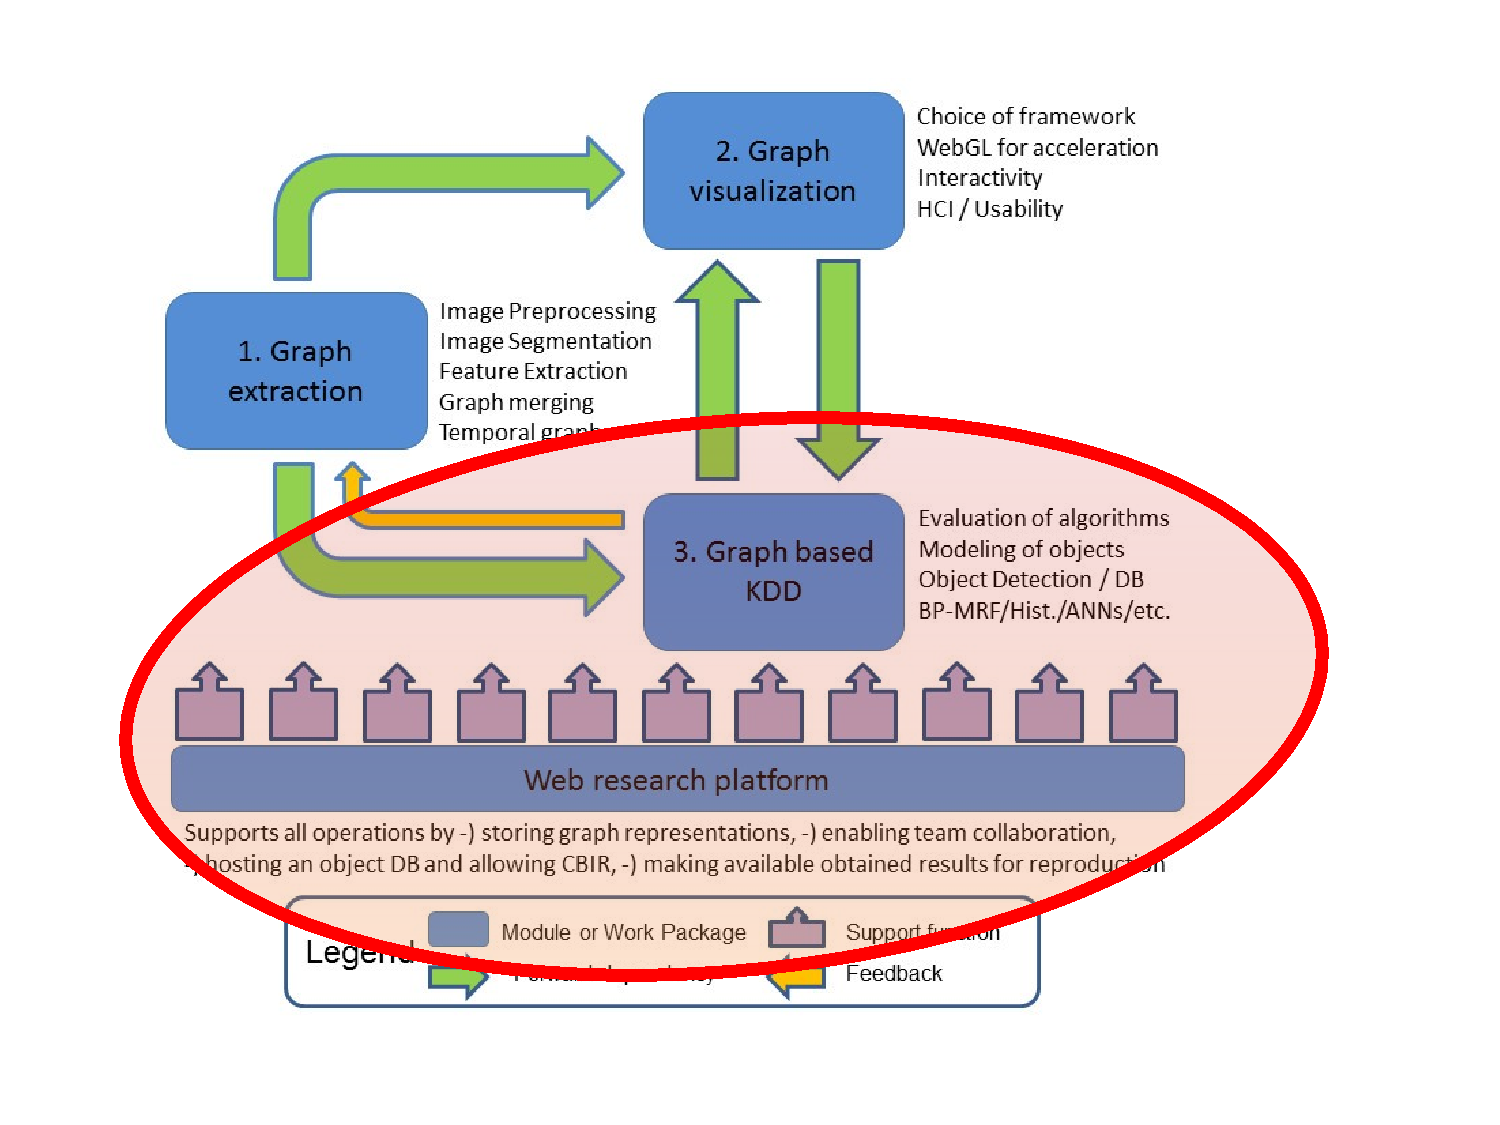
\includegraphics[width=1.1\textwidth]{figures/iKNOdis_OGMA_structure}
	\caption{Former project iKNOdis architecture overview}
	\label{fig_iKNOdis_structure}
	\small
	Whereas iKNOdis.net was meant to be used exclusively for image processing via graph-theoretical approaches, we broadened the idea of application areas while reducing the aim for specific scientific advances in image processing. The result is a Web-based, graph-theoretical processing platform whose base functionality (an in-browser graph library called GraphiniusJS) as well as visualization capabilities (GraphiniusVIS) are the main subjects of the Master Thesis at hand.
\end{figure}

In the process of creating an FWF proposal out of iKNOdis, the project was split into two separate endeavors in order to make them amenable to independent, smaller funding efforts as well as enabling separate groups of developers to work on their respective areas of interest. This resulted in the formation of project Graphinius covering all graph-theoretical aspects and basic data-engineering infrastructure \cite{DataAnalysisDSWorkflow} by providing a Browser based graph processing and visualization platform.

As a side-effect, Graphinius follows no specific research goal itself; we rather envision it as a future engineering infrastructure for data scientists, may they concern themselves with Machine Learning, Biomedical applications or any other field. This mental 'expansion' to a diverse set of interesting areas of application is reflected by an in-depth discussion of several potential candidates in Chapter~\ref{ch:theory_applications} as well as 3 different demo applications described in Chapter~\ref{ch:impl_aoa}.

As evolution (of ideas) never stops, there are already new ideas springing up concerning the future of Graphinius - the most obvious one regarding a spin-off company providing the platform as a hosting service for the community - such a startup could profit from several different advantages over its competitors. Second, GraphiniusJS alone (without integration into the larger platform) could power web applications of the future (see Section~\ref{ssect:the_local_sphere}), enabling graph-based recommender systems for social networks that could be truly organized as \textit{peer networks} - without or with only a minimal server infrastructure.


\section{How this thesis is structured}
\label{section:thesis_structure}

The rest of this chapter is composed of a short description of how scientific computing / machine learning tasks are handled today. We will explore the benefits individual users as well as the whole research community could derive from conducting experiments on such a platform; therefore we have to outline potential properties and focal points of the proposed technology.

In Chapter~\ref{ch:theory_applications}, Theoretical background / applications we are introducing different potential areas of application for Graphinius. The reader will notice that practically all of the fields discussed may be of interest to researchers outside the 'hardcore' Machine Learning or Data Science communities.

Chapter~\ref{ch:business_case} deals with possible economic opportunities involving the Graphinius platform and its conceivable business model, and will discuss some potential competitors.

An outline of the basic functionality of Graphinius will be given in Chapter~\ref{ch:graphinius_platform}, comprising technical features, graph-theoretical design decisions as well as handling characteristics important to its users.

The modern web development process will be discussed in-depth in Chapter~\ref{ch:software_requirements}, where we will become acquainted 
with a set of requirements for modern Web based software and then go on to explore suitable technologies in each category and compare them to one another. At the end of this chapter, we will have all the tools in our hand to start building Graphinius.

I will go into details about the project implementation in Chapter~\ref{ch:implementation}, introducing each relevant subsystem in sequence, pointing out its role in the larger context and explain how and why it was built the way it was built.

In Chapter~\ref{ch:impl_aoa} the reader will find three demo applications that have been implemented on top of Graphinius as a proof of feasibility of the platform. I will introduce some specific (mathematical) background knowledge and provide the sample results obtained using Graphinius.

Chapter~\ref{ch:results_discussion} will provide some structural as well as performance metrics about the Graphinius (JS) library and (proudly) present the test coverage achieved as of the date of this writing.

Taking a look into the future in Chapter~\ref{ch:future_work}, we will discuss some promising new concepts and technologies which hold great potential for the advancement of any Web based, community-oriented research platform.

I will finish this thesis with a summary and conclusion in Chapter~\ref{ch:conclusion}, and give some additional information about anonymization outputs in Appendix~\ref{App:AppendixA} and provide the whole Graphinius API as of the time of this writing in Appendix~\ref{App:AppendixB}.


\section{How Machine Learning / KDD are approached today}
\label{sect:ml_kdd_today}

When i was taking the famous Machine Learning MOOC tought by Prof. Andrew Ng from Stanford University on Coursera in 2013, one story he conveyed during a section on optimizing Machine Learning Pipelines had especially caught my attention. As a specialist in high demand Prof. Ng is frequently consulting for Silicon Valley companies in matters of Machine Learning and Artificial Intelligence. On one of these occasions, the client company had been trying to optimize their ML pipeline for the better parts of 2 years without any significant improvements in their results. After looking at the different stages of their pipeline and conducting a so-called ceiling analysis, Prof. Ng concluded that two developers had spent 18 months on optimizing their background separation algorithm while the most significant potential for improvement really lay in a latter stage of the process. Based on this analysis the company was able to remedy the shortcomings in a relatively short period of time.

\par

This incident shows how much effort is potentially squandered by trying to implement sophisticated algorithms within isolated teams in a non-standardized fashion: Proprietary approaches - both in technology as in methodology - hinder the exchange of information with other members of the research community, thus opening up vulnerabilities to making mistakes which could have easily been avoided by considering the experience of other professionals. The following properties of data analysis / ML projects seem to give rise to such vulnerabilities:

\begin{itemize}
	\item \textbf{Isolation.} Working on common machine learning problems in isolated teams without communication makes comparison of approaches as well as results unnecessarily hard. Dealing with errors at any stage of the algorithmic pipeline takes more effort than necessary due to a lack of reference values, while achieving superb results has little to no effect on the potential of other projects.
	\item \textbf{Proprietary Software.} Countless professionals prefer developing data analysis pipelines in highly proprietary software environments like Matlab or Mathematica. This prevents an influx of solid, community-tested algorithms while preventing others from gaining knowledge acquired in such organizations (as long as they are unwilling to pay horrendously for the software).
	\item \textbf{Irreproducibility.} As unpublished code cannot be perfectly reverse engineered, experiments conducted in isolation can't be easily corroborated. This might be advantageous with respect to product development and patent procedures, but is usually detrimental to the efforts of researchers trying to get published and spreading their insights.
	\item \textbf{Lack of scalability.} Last but not least, heterogeneous and highly customized data processing pipelines might not lend themselves well to parallelization, which might prevent the use of such algorithms on quickly expanding datasets.
\end{itemize}

This leads us to the insight that a readily available (no complex setup or configuration), public and open source, standardized and scalable infrastructure which promotes the cross-fertilization of ideas and insights from individual experiments, would form the ideal model of a future, successful Machine Learning platform (graph-theoretical or otherwise).


\section{How a Web based approach could benefit users, researchers and society}
\label{sect:web_benefits}

Over the past several years, many platforms have emerged in the realm of \textit{data engineering}, providing means for researchers and data professionals to easily learn, deploy and scale machine learning models 
\cite{DataScienceTools2013}. The greatest disadvantage of those platforms however, is that they all target the tech-savvy programming experts and experienced system administrators. While this may not be a problem for core ML researchers and programmers, it presents a serious obstacle to experts in the Life Sciences etc.

Second, most modern frameworks allow for the setup of huge and very efficient clusters on a hardware / filesystem virtualization level. They do not provide built-in community networking functions, however, which could bridge the experience gap between disciplines (e.g. via hyper heuristics) or allow for easy reproducibility of results. The following list shall give a short overview of potential advantages of the Graphinius Platform:

\begin{itemize}
	\item \textbf{Ease of access.} With configuration and loading of binaries happening automatically from the outside, barely any costs for technical configuration and conducting experiments arise.
	
	\item \textbf{Effortless scalability} As users of the platform provide their own computing power via their browsers, the server role can initially be reduced to that of a static document server / database server.
	
	\item \textbf{Automatic grid potential.} As browsers were intended to always be connected to a larger network of computers, and 2-way communication via Web Sockets has recently become commonplace, we can imagine the JavaScript Virtual Machine (JSVM) as a natural node of a dynamic virtual grid computer - akin to a client node in Berkeley's BOINC framework (Seti@Home).
	
	\item \textbf{Centralization of experiment meta data.} As code and configuration will be stored and transmitted by a Web servers anyways, nodes will be able to send descriptions of conducted experiments back to the servers for storage and evaluation. Given enough participants on the platform, this would lead to the formation of ML meta knowledge, as to which algorithms in what sequence would perform best given some inputs and specified problem class (prediction, description, ...).
	
	\item \textbf{Hyper Heuristics} are a way of selecting or configuring algorithms by searching a space of lower level heuristics instead of searching the solution (or parameter) space itself. Hyper heuristics are different from Meta Learning in that they work independent of the problem domain and therefore promise to be generally applicable; the challenges lie in producing algorithms with a good overall runtime behavior - therefore, meta-data about experiments from diverse problem domains are required.
	
	\item \textbf{A Pipeline recommender} with the ability to automatically instantiate and execute the recommended (sequence) of algorithms could be built upon this knowledge, which would further enhance a researcher's capacity to conduct more experiments faster, potentially leading to an increase in frequency or quality of scientific output.
	
	\item \textbf{Instant deployment.} In traditional scientific programming, there is a large gap between developing a model suitable for a specific research question and actually deploying it in a production environment \citep{AnalLifecycle}. Being Web based, Graphinius' development and production environment are one and the same, reducing the deployment procedure to posting a link to an experiment (for scalability, see above).
	
	\item \textbf{Great visual capabilities.} Although there exist great visualization toolkits for many of the data science platforms out there today, the sheer mass of 2D and 3D libraries running in the browser enable completely new ways to demonstrate, interact with, and even manipulate results in real time. Moreover, exchanging of 'live' results (via simple bookmarks) instead of 'dead' graphs (in scientific papers) would soon become standard amongst members of such a community.
\end{itemize}
